\documentclass{ctexart}

\usepackage{amsmath}
\usepackage{amssymb}
\usepackage{amsfonts}
\usepackage{listings}
\usepackage{tikz}
\usetikzlibrary{automata,positioning}

\usepackage{color}

\definecolor{mygreen}{rgb}{0,0.6,0}
\definecolor{mygray}{rgb}{0.5,0.5,0.5}
\definecolor{mymauve}{rgb}{0.58,0,0.82}

\lstset{ %
	backgroundcolor=\color{white},   % choose the background color; you must add \usepackage{color} or \usepackage{xcolor}
	basicstyle=\footnotesize,        % the size of the fonts that are used for the code
	breakatwhitespace=false,         % sets if automatic breaks should only happen at whitespace
	breaklines=true,                 % sets automatic line breaking
	captionpos=b,                    % sets the caption-position to bottom
	commentstyle=\color{mygreen},    % comment style
	deletekeywords={...},            % if you want to delete keywords from the given language
	escapeinside={\%*}{*)},          % if you want to add LaTeX within your code
	extendedchars=true,              % lets you use non-ASCII characters; for 8-bits encodings only, does not work with UTF-8
	frame=single,	                   % adds a frame around the code
	keepspaces=true,                 % keeps spaces in text, useful for keeping indentation of code (possibly needs columns=flexible)
	keywordstyle=\color{blue},       % keyword style
	language=Octave,                 % the language of the code
	otherkeywords={*,...},           % if you want to add more keywords to the set
	numbers=left,                    % where to put the line-numbers; possible values are (none, left, right)
	numbersep=5pt,                   % how far the line-numbers are from the code
	numberstyle=\tiny\color{mygray}, % the style that is used for the line-numbers
	rulecolor=\color{black},         % if not set, the frame-color may be changed on line-breaks within not-black text (e.g. comments (green here))
	showspaces=false,                % show spaces everywhere adding particular underscores; it overrides 'showstringspaces'
	showstringspaces=false,          % underline spaces within strings only
	showtabs=false,                  % show tabs within strings adding particular underscores
	stepnumber=1,                    % the step between two line-numbers. If it's 1, each line will be numbered
	stringstyle=\color{mymauve},     % string literal style
	tabsize=2,	                   % sets default tabsize to 2 spaces
	title=\lstname                   % show the filename of files included with \lstinputlisting; also try caption instead of title
}

\lstdefinestyle{customc}{
	belowcaptionskip=1\baselineskip,
	breaklines=true,
	frame=L,
	xleftmargin=\parindent,
	language=C,
	showstringspaces=false,
	basicstyle=\footnotesize\ttfamily,
	keywordstyle=\bfseries\color{green!40!black},
	commentstyle=\itshape\color{purple!40!black},
	identifierstyle=\color{blue},
	stringstyle=\color{orange},
}

\lstdefinestyle{customasm}{
	belowcaptionskip=1\baselineskip,
	frame=L,
	xleftmargin=\parindent,
	language=[x86masm]Assembler,
	basicstyle=\footnotesize\ttfamily,
	commentstyle=\itshape\color{purple!40!black},
}

\lstset{escapechar=@,style=customc}

\begin{document}

\section*{Problem 1.6}
Show that the set of all finite subsets of an enumerable set is enumerable.

Solution:

Let $\mathcal S = \{ s_1, s_2, \dots, s_k \}$ be a subset of the enumerable set $\mathbb S$. Since $\mathbb S$ is enumerable, there is $f: \mathbb S \to \mathbb Z^+$ such that $f(s_i) = z_i$, where $ 1 \le i \le k$. Encode every element of $\mathcal S$ we have
$$
\mathcal D = \{ d_1, d_2, \dots, d_k\}
$$
where $d_i$ is positive integer, with $1 \le i \le k$.

Encode $\mathcal D$ with $(k, a) = (k, G_k(\mathcal D))$, where
$$
G_k(\{ d_1, d_2, \dots, d_k\}) = G_2(d_1, G_{k-1}(d_2, d_3, \dots, d_k))
$$
where $G_2(m, n) = \frac{(m + n - 1)(m + n - 2)}{2} + m$, then encode $(k, a)$ with $o = G_2(k, a)$.

\section*{Problem 2.1}
Show that the set of all subsets of an infinite enumerable set is nonenumerable.

Solution:

Define matrix $A$
$$
A(i, j) = \begin{cases} 1 & E_j \in S_i \\ 0 & E_j \not\in S_i \end{cases}
$$

where $E$ is the infinite enumerable set, and $S$ is the set of all subsets of $E$.

Define set $S' = \left\{ E_i \mid A(i, i) = 0 \right\}$. Assuming $S' = S_i \in S$, if $A(i, i) = 1$, then $E_i \in S_i$ but $E_i \not\in S_i$; if $A(i, i) = 0$, then $E_i \not\in S_i$ but $E_i \in S_i$. Thus, the set of all subsets of an infinite enumerable set is nonenumerable.

\section*{Problem 2.11}
Show that the set of points on a line is equinumerous with the set of points on
a plane.

Solution:

We can easily map any point $x$ in a line to $[-\pi, \pi]$ with $f(x) = \arctan(x)$, then let $g(f(x)) = \frac{f(x) + \pi}{2\pi} \in [0, 1]$. We can also map a point $y$ in $[0, 1]$ to any point $x$ with $x = f'(g'(y))$, where $g'(y) = 2\pi \times y - \pi$, and $x = f'(g'(x)) = \tan(g'(y))$.

Similarily, a point $(a, b)$ on a plane can be map to $(f(g(a)), f(g(b)))$, where $f(g(a)) \in [0, 1]$ and $f(g(b)) \in [0, 1]$, and vice versa.

Finally, we can map a point $0.a_1 b_1 a_2 b_2 \dots$ in $[0, 1]$ to point $(0.a_1 a_2 \dots, 0.b_1 b_2 \dots)$. Vice versa, we can map point $(0.a_1 a_2 \dots, 0.b_1 b_2 \dots)$ to $0.a_1 b_1 a_2 b_2 \dots$. Thus, the points on a line segment is equinumerous with the set of points on a square.

Since all these 4 sets are equinumerous, the set of points on a line is equinumerous with the set of points on a plane.

\section*{Problem 3.4}
Design a Turing machine that, starting with the tape as in the preceding problems, will eventually halt on the leftmost stroke on the tape, which is now to contain a block of n strokes, followed by a blank, followed by a block of m − 1 strokes, followed by a blank, followed by a block of k strokes.

Solution:

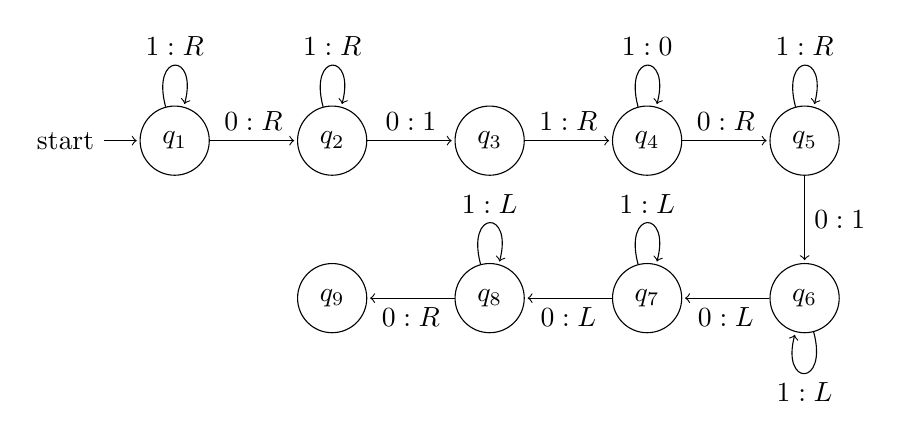
\begin{tikzpicture}[shorten >=1pt,node distance=2cm,on grid,auto] 
\node[state,initial] (q_1) {$q_1$};
\node[state] (q_2) [right=of q_1] {$q_2$};
\node[state] (q_3) [right=of q_2] {$q_3$};
\node[state] (q_4) [right=of q_3] {$q_4$};
\node[state] (q_5) [right=of q_4] {$q_5$};
\node[state] (q_6) [below=of q_5] {$q_6$};
\node[state] (q_7) [left=of q_6] {$q_7$};
\node[state] (q_8) [left=of q_7] {$q_8$};
\node[state] (q_9) [left=of q_8] {$q_9$};
\path[->]

(q_1) edge node {$0:R$} (q_2)
edge [loop above] node {$1:R$} ()
(q_2) edge node {$0:1$} (q_3)
edge [loop above] node {$1:R$} ()
(q_3) edge node {$1:R$} (q_4)
(q_4) edge node {$0:R$} (q_5)
edge [loop above] node {$1:0$} ()
(q_5) edge node {$0:1$} (q_6)
edge [loop above] node {$1:R$} ()
(q_6) edge node {$0:L$} (q_7)
edge [loop below] node {$1:L$} ()
(q_7) edge node {$0:L$} (q_8)
edge [loop above] node {$1:L$} ()
(q_8) edge node {$0:R$} (q_9)
edge [loop above] node {$1:L$} ()
;
\end{tikzpicture}

\section*{3.6}
Design a Turing machine to compute the function max(x, y) = the larger of x and y.

Solution:

\begin{lstlisting}[frame=single]
write 1; // set central pivot
move left; // left arg reduce 1
write 0;
move left;
if (0) move right; else goto (10);
move right;
write 0;
move right;
halt;
move right;
move right; // back to central pivot
move right; // right arg reduce 1
write 0;
move right;
if (0) move left; else goto (23);
move left;
write 0;
move left;
write 1;
while (1) move left; // point to left number
move right;
halt
move left;
move left; // back to central pivot
move left; // scan left, reduce 1
while (0) move left;
write 0;
move left;
if (0) move right; else goto (37);
while (0) move right; // left number smaller
write 0;
move right;
while (0) write 1; move right;
while (1) move left;
move right;
halt;
move (0) move right; // back to pivot, scan right
move right;
while (0) move right;
write 0;
move right;
if (0) move left; else goto (50);
while (0) move left; // right number smaller
write 0;
move left;
while (0) write 1; move left;
while (1) move left;
move right;
halt;
move left;
while (0) move left;
goto (25);
\end{lstlisting}

\section*{Problem 4.1}
Is there a Turing machine that, started anywhere on the tape, will eventually halt if and only if the tape originally was not completely blank? If so, sketch the design of such a machine; if not, briefly explain why not.

Solution:

Idea: Repeat searching left then right, set `1` as marker. Corresponding automaton:

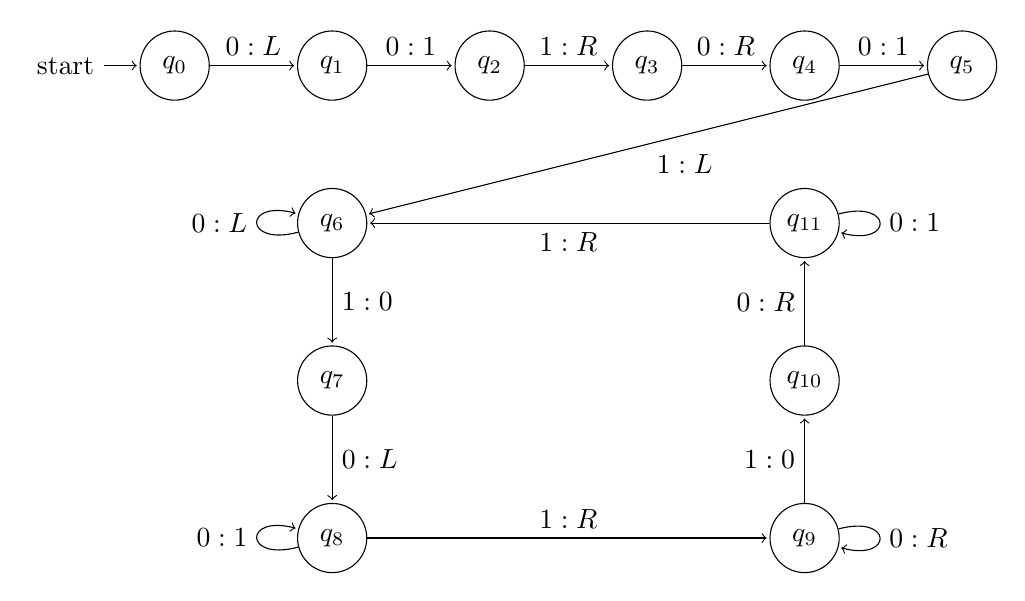
\begin{tikzpicture}[shorten >=1pt,node distance=2cm,on grid,auto] 
\node[state,initial] (q_0) {$q_0$};
\node[state] (q_1) [right=of q_0] {$q_1$};
\node[state] (q_2) [right=of q_1] {$q_2$};
\node[state] (q_3) [right=of q_2] {$q_3$};
\node[state] (q_4) [right=of q_3] {$q_4$};
\node[state] (q_5) [right=of q_4] {$q_5$};
\node[state] (q_6) [below=of q_1] {$q_6$};
\node[state] (q_7) [below=of q_6] {$q_7$};
\node[state] (q_8) [below=of q_7] {$q_8$};
\node[state] (q_11) [below=of q_4] {$q_{11}$};
\node[state] (q_10) [below=of q_11] {$q_{10}$};
\node[state] (q_9) [below=of q_10] {$q_9$};
\path[->]

(q_0) edge node {$0:L$} (q_1)
(q_1) edge node {$0:1$} (q_2)
(q_2) edge node {$1:R$} (q_3)
(q_3) edge node {$0:R$} (q_4)
(q_4) edge node {$0:1$} (q_5)
(q_5) edge node {$1:L$} (q_6)

(q_6) edge node {$1:0$} (q_7)
edge [loop left] node {$0:L$} ()
(q_7) edge node {$0:L$} (q_8)
(q_8) edge node {$1:R$} (q_9)
edge [loop left] node {$0:1$} ()

(q_9) edge node {$1:0$} (q_10)
edge [loop right] node {$0:R$} ()
(q_10) edge node {$0:R$} (q_11)
(q_11) edge node {$1:R$} (q_6)
edge [loop right] node {$0:1$} ()
;
\end{tikzpicture}

\begin{lstlisting}[frame=single]
if (current is 1) halt
move left;
if (current is 1) halt; else write 1; // left boundary
move right;
move right;
if (current is 1) halt; else write 1; // right boundary
move left; // center pivot;
while (current is 0) move left; // goto left boundary
write 0;
move left;
if (current is 1) halt; else write 1;
move right;
while (current is 0) move right; // goto right boundary
write 0;
move right;
if (current is 1) halt; else write 1;
move left;
goto (8);
\end{lstlisting}

\end{document}